\subsection{Prospective local inhibitory-context gating in the conductance tree}
\label{note:conductance_local_gate}

This follow-up used the same directed identity-output E/I tree as the preceding opponent-tuning comparison. Its protocol was fixed and committed before the new runs, after exposure to a referee panel's exploratory tests of local gating. Those panel outcomes and the historical seed used for numerical replay are excluded from every new scientific summary. Twenty fresh seed blocks, 2026090801--2026090820, pair teacher perturbations, initial weights, inputs, contexts and minibatch sequences across the two tasks and all conditions.

For terminal compartment $j$ with proximal parent $p(j)$, the primary rule supplies $\widehat\delta_j=\delta\mathbf1[a_{p(j)}=0]$, where $\delta$ is the somatic loss derivative and $a_p$ is externally supplied inhibitory activity, either zero or ten. Both proximal compartments and the soma retain multiplier one. No exact path derivative or oracle projection is evaluated in the local rule's gradient computation. The sixteen terminal gains, two proximal inhibitory gains, four daughter couplings and two soma couplings all retain their exact local eligibility derivatives with respect to log conductance. Student terminal gains are nominally one. Other nominal values are proximal inhibition 15, daughter couplings $(20,0.2)$ within each subtree, and soma couplings four. Every student log gain receives a separate Gaussian SD~0.4 perturbation; teacher log perturbations have SD~0.15. Thus students share an informed nominal scaffold, but not the teacher's realized weights.

The nine rules are exact credit, unit broadcast, an initially calibrated profile, a three-pattern oracle projection, the hard distal gate, its swapped version, the gate extended to proximal credit, a two-leaf-pattern oracle with unit proximal credit, and a continuous local inhibitory-conductance gate. Calibration averages initial exact path factors over 512 independent unlabeled examples. The three disjoint weighted columns address leaves $(0,1)$, leaves $(2,3)$ and proximal units $(4,5)$ in the implementation's indexing. Their coefficients project the current exact field. The two-leaf control uses the same two distal projections but supplies unit proximal multipliers; it must not be interpreted as an entirely rank-two six-site dictionary or as a locally learned encoder. The continuous local gate multiplies terminal credit by $[1+g_{\mathrm I,p}a_p]^{-1}$ and leaves proximal and somatic credit unchanged. Its denominator contains the local open inhibitory conductance, not the exact downstream path gain.

The proximal-gating control exposes a specific eligibility interaction. The local derivative of proximal voltage with respect to its inhibitory log gain is proportional to $-a_pV_pg_{\mathrm I,p}/D_p$, where $D_p$ is total proximal conductance. It is nonzero only when $a_p>0$. Multiplying its credit by $\mathbf1[a_p=0]$ therefore makes this parameter's gradient identically zero. Both inhibitory gains remain frozen in all such trajectories. This control retains 24 parameter slots but does not preserve effective plasticity of all 24. Gating only terminal credit avoids this failure.

Each teacher/task provides 2,048 training, 1,024 validation, 4,096 test, 512 calibration and 1,024 diagnostic examples, with no added label noise. Adam uses rates 0.01, 0.03 and 0.1, $\beta_1=0.9$, $\beta_2=0.999$, $\epsilon=10^{-8}$, no weight decay, 128-example minibatches, global gradient clipping at ten and log-conductance bounds $[-7,7]$. Rate 0.03 is the primary fixed rate; the other two rates are symmetric robustness conditions, not candidates selected from fresh outcomes. The full design comprises $20\times2\times9\times3=1,080$ initialized trajectories. All continue without resetting parameters, optimizer or minibatch state to 16,384 updates. Minimum validation loss within 4,096 and 16,384 updates selects two endpoint views of each trajectory. Fixed-step endpoints and every recorded checkpoint are retained.

The primary opposed-task unit-broadcast-minus-local-gate NMSE was 0.48737 (95\% paired interval, 0.35763--0.61447). Subtracting the aligned-task gap gave 0.48683 (0.36027--0.61475). Both differences were positive in all twenty seeds; two exact two-sided sign-flip tests each gave $P=1.907\times10^{-6}$ and Holm-adjusted $P=3.815\times10^{-6}$. At 16,384 updates the task-by-rule interaction was 0.46815 (0.33207--0.60392), again positive in all twenty seeds. Intervals use 20,000 whole-seed bootstrap resamples; secondary rates, rules and budgets are descriptive.

At the primary budget, hard-minus-exact opposed NMSE was $1.49\times10^{-6}$ ($-1.60\times10^{-6}$ to $4.86\times10^{-6}$). The maximum hard-gate NMSE was $5.47\times10^{-5}$. These satisfy the prespecified practical references of an upper paired interval below 0.001 and every seed below 0.01, without establishing asymptotic equivalence. The two-leaf oracle and proportional local rule achieved mean opposed NMSEs $2.28\times10^{-5}$ and $2.32\times10^{-5}$. Reversing selection gave 0.94926; gating proximal credit as well gave 0.12320, with nineteen of twenty seeds above 0.01. Both effects remained at the longer budget. All hard-distal fits at all three rates changed all 24 parameters and reached low error. No primary-rate exact, hard-distal, projected or proportional fit contacted the parameter bounds through 16,384 updates. Broadcast and failed-gate controls did contact bounds; all trajectories had zero gradient-norm clipping. These remain finite-bound and finite-budget comparisons.

Ten mechanism tests establish finite-difference gradient agreement, reference-adapter agreement, preservation of proximal eligibility, the proximal-inhibition failure identity, and absence of exact-path access in local gradient code. An excluded replay of both tasks on historical seed 2101 reproduces 4,096-update exact, unit and calibrated parameter/optimizer trajectories bit for bit. The independently evaluated three-column projection differs by at most $3.73\times10^{-14}$ in saved parameters and $1.56\times10^{-17}$ in checkpoint NMSE. Resolved configurations, initial/input/checkpoint hashes, bounds, all seed endpoints and the committed protocol are supplied under \texttt{source\_data/conductance\_local\_gate/}. Standalone replay writes to a separate directory and does not require a Git checkout.

\begin{figure}[p]
\centering
% Root integration supplies the canonical supplementary figure filename.
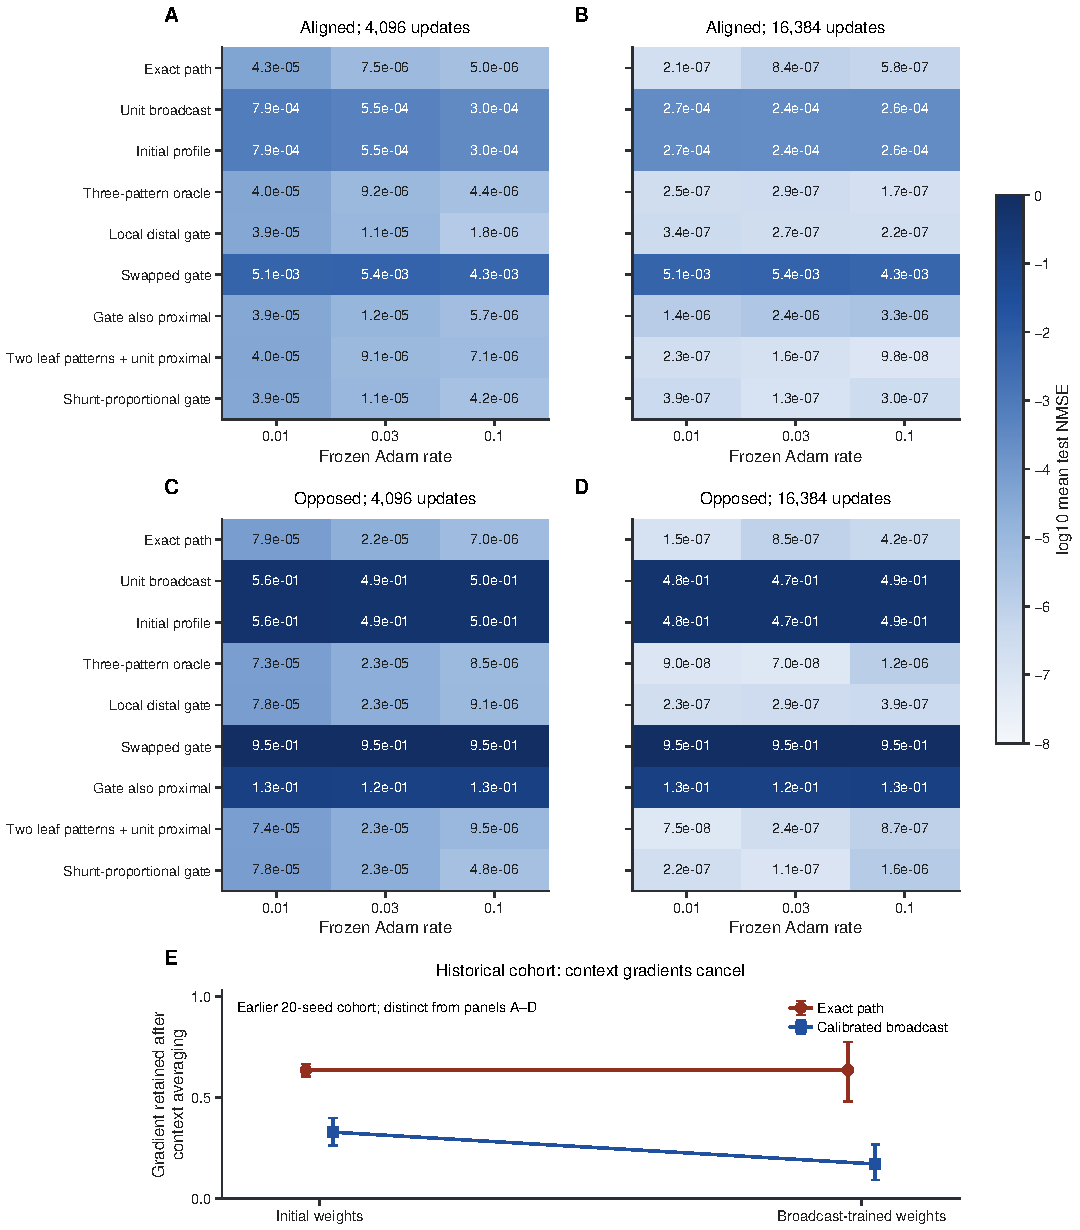
\includegraphics[width=\textwidth]{../source_data/conductance_local_gate/figures/local_gate_all_rates.pdf}
\caption{\textbf{Complete local-gate controls and the earlier cancellation diagnostic.} \textbf{A,B}, Aligned task at 4,096 and 16,384 updates. \textbf{C,D}, Opposed task at the same budgets. Entries are mean held-out NMSE across twenty fresh paired seed blocks, using the checkpoint with lowest validation NMSE within the stated budget. Every rule receives every frozen rate; rate 0.03 is primary and no fresh outcome selects a new rate. Color reports $\log_{10}$ mean NMSE on the same scale across panels. The two-leaf and three-pattern controls use oracle coefficients; the hard and proportional local gates do not. All 1,080 trajectories and both endpoint windows are retained, with detailed seed values and parameter-bound accounting in Source Data. \textbf{E}, Historical context-gradient diagnostic from the preceding twenty-seed cohort (seeds 2101--2120), distinct from the fresh cohort in \textbf{A--D}. At initial and broadcast-trained weights on the opposed task, exact and calibrated-broadcast credit are evaluated with the same weights, inputs and local eligibilities. The ordinate is the norm of the context-averaged distal gradient divided by the context-weighted sum of conditional gradient norms, before Adam: zero denotes complete cancellation and one denotes none. Points and whiskers are means and descriptive 95\% seed-bootstrap intervals. This panel retains the earlier mechanism illustration; it does not measure gradients from the new local-gate fits.}
\label{fig:supp_local_gate_rates}
\end{figure}
